
\documentclass[12pt]{article}
\usepackage[margin=1in]{geometry}
\usepackage[pdftex]{graphicx}
\usepackage{multirow}
\usepackage{setspace}
\usepackage{enumitem}
\pagestyle{plain}

\begin{document}

% Course information
\begin{tabular*}{\textwidth}{l @{\extracolsep{\fill}} r}
  & \multirow{3}{*}{
\includegraphics[height=1.0in]{logo.jpg}} \\
  \large Experimental Techniques & \\
  \large Winter Quarter 2020 & \\
  \large Physics 80 & \\
\end{tabular*}
\vspace{10mm}

% Professor information
\begin{tabular}{ l l }
  \multirow{6}{*}{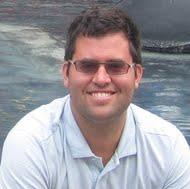
\includegraphics[height=1.25in]{mike.jpg}} & \\
  & \\
  & \large Michael Mulhearn \\
  & \large mulhearn@physics.ucdavis.edu \\
  & \large Physics 317 \\
  & \\
\end{tabular}
\vskip 0.5cm
\noindent
\textbf {Lectures:} M,W 11:00-11:50 PM in Giedt 1006
\begin{tabbing}
\hspace*{3em}\= \hspace*{5em} \= \kill % set the tabbings
\textbf {Lab:}    \> Section 1: \> M,W 12:40-3:00 PM in Rm. 152 Roessler (changed!)\\
                  \> Section 2: \> T,R 3:10-5:30 PM in Rm. 152 Roessler \\
\end{tabbing}


\noindent
\textbf {Text:}  Online lecture notes at {\tt https://www.scipy-lectures.org} plus
lecture notes on RLC circuits and Data Analysis on the course website. \\

\noindent
\textbf{Office Hours:} M 12:00-1:00 PM in Rm. 152 Roessler\\

\noindent
\textbf{Lab Instructor:} Andrew Diggs (amdiggs@ucdavis.edu) \\

\noindent
\textbf {Course Description:}  
This course is an introduction to experimental laboratory techniques
and data analysis.  Laboratory techniques include electronics circuits
and optical systems and related test equipment.  Data analysis based
on scientific python includes statistical and systematic analysis,
curve fitting, and noise.\\

\noindent
\textbf{Homework:} 
There will be approximately five homework assignments, based on the
lecture material.  Do not post the problems to internet forums.  To
minimize the effectiveness of cheating, homework scores will be based
solely on whether a legitimate attempt was made.  The best way to
prepare for the exams and the quizzes is to solve problems yourself or
by actively participating within a study group.  Always be prepared to
explain your work.  Homework and due dates will be posted on the course website.\\

\noindent
\textbf{Quizzes:}  There will be occasional low-stakes single-problem quizzes during lecture, based on the homework.\\

\noindent
\textbf{Midterm Exam:} Tue, 29 Jan during lecture \\

\noindent
\textbf{Final Exam:} Tue, 17 March at 8:00 AM in 1006 Giedt \\

\newpage

\noindent
\textbf {Lab Safety:}\\
You should complete the online course for Electrical Safety at \\
{\tt http://safetyservices.ucdavis.edu/training/electrical-safety}.\\
You should also read your lab descriptions carefully, and ask your TA if you have any concerns about safety.\\

\noindent
\textbf {Labs:}\\
The lab portion of this class is the most important.  You are expected
to attend every lab session.  You should come to each lab well
prepared, having read through the lab write-up ahead of time, with a
clear plan in mind.

With the exception of scheduled make-up lab at the end of the course,
there is no opportunity to make-up labs that are missed.  There is
also one catch-up lab where you can finish any of the early labs that
were not completed.  In addition to the make-up lab, your worst lab
score (and any related logbook or notebook scores) will be dropped
from your final grade.  This covers one full week of absence from the
class.  Also, you must complete the Planck's constant lab, the speed
of light in air lab, and the muon lifetime lab by the end of course.
If you miss one of these labs, you must make it up during the final
make-up lab.  The second section of lab generally goes smoother than
the first, and so lab scores for the second section may be inflated to
account for this.

For each lab, you will be assigned a score from 1 to 10 based on the
TA's assessment of your performance in the lab that day based on the
following criteria:
\begin{itemize}
\item {\bf Attendance} will be taken at the start of lab. Check-in
  with the TA if you arrive late.
\item {\bf Technical Questions} will be asked to specific students as
  the TA circulates the room.  At all times, you should be able to
  explain each connection in your setup and each line in your code.
  Do not answer questions posed to your lab partner, as this prevents
  the TA from assessing you separately.
\item {\bf Professional Attitude} will be evaluated by the TA by watching your interactions with your lab partners and other queues.  Lab work requires your undivided attention, curiosity, and active participation.  
\item {\bf Independence} is an important trait for making progress in research.  Your TA is available to help and answer questions, but you should make every effort to figure things out for yourself.  You will find in life that people are much more willing to help when your question makes it clear that you made an informed and competent attempt at doing it yourself first.
\item {\bf Neatness} of your setup will be evaluated.  Generally the neatest circuits are the ones that finish first.  Think about layout, and use short loops of wire to connect things.  Use a consistent color scheme for the wires in you circuit.  Trim components if the leads are unwieldly.
\end{itemize}
Flawless performance in the lab is an 8.  For scores of 7 and below,
you can ask the TA for specific commentary on what you were ``dinged''
for.  This is the most subjective score in the course, but it is
included in your grade to encourage you to think about and develop
these traits.

Most scientist these days employ a mixture of handwritten and digital
logbooks.  Quick notes and sketches about procedures, calculations,
and the results of simple measurements are often most conveniently
handwritten.  Extensive data collection and detailed analysis are
usually done entirely on a computer.  This course includes a
hand-written logbook and Jupyter Notebooks.  The introduction of each
lab indicates which of these will be used in the lab (either one or
both).\\

\noindent
\textbf {Logbooks:}\\ 
Each student must provide their own handwritten logbook which remains
at all times in the lab.  Professional logbooks are expensive, but for
this course you may use an inexpensive ``Graph Ruled Composition''
notebook as a decent approximation.  The instructor will bring an
example to the first lecture, and you will not need your logbook until
the second week of class.  {\bf Do not take your logbook out of the
  lab.}\\

You should write in pen, not pencil.  You logbook should include:
\begin{itemize}
\item Title of the lab, date and names of your lab partners.  
\item Dates (and times) liberally spread throughout the data/figures/narratives.
\item Page numbers. Add sequential numbers for all the pages in your logbook. 
\item Present things in a neat, legible and organized way.
\item Sketches of the apparatus and of important details of the apparatus, even when we provide you with those in the lab manual.
\item Data: numbers, examples of your signal, comments and descriptions, systematically entered (in tabular form where possible). All the data should be there, including the data that failed (with annotation of why it failed). 
\item Entries like "Measurement 1.1" in the lab manual indicate entries you should enter in your logbook. Mark the entry in your logbook accordingly, i.e. "Measurement 1.1:".
There should be a sketch of your apparatus associated with each measurement, but you can reuse sketches from previous measurements (e.g. "Same configuration as in Measurement 2.1 but with R1 = 1 kOhm")
\item Preliminary analysis, calculations and uncertainty estimates based on the data.
You should always check your data as best you can while taking it, to make sure that you are not wasting time taking non-sensible data.  These sort of checks belong in your logbook, even if the final complete analysis is done in python.  (You can also note that you plotted things in python and they looked OK.)
\item Comments in response to direct questions posed in the lab manual, or simply to record things you observed.
\end{itemize}

Most labs include one or more {\bf Sign-Off Points}.  At these points,
you should let the TA witness your accomplishment and sign your
logbook. After notifying the TA, if the TA is busy, move on with the
lab, leaving the setup intact or easily reproducible if possible.

At several points during the quarter, the TA will skim your logbook
and offer feedback and a score on a 10 point scale, based on the
criteria above, and the amount of each lab completed.\\

\noindent
\textbf {Jupyter Notebooks:}\\ 
The analysis portion of this lab will be completed with Scientific
Python in Jupyter Notebooks, installed on the lab PCs.  You may also
choose to install Scientific Python on your own laptop, it is a very
handy tool, and freely available for any major OS.

Place the name of the lab, the date of the lab, and the name of all of
your lab partners in the first cell as a comment, even if you are each
keeping your own notebook.

Start each of your notebooks with the magic python function
{\tt\%pylab inline} to load numpy as np, matplotlib as plt, and show
plots as cell output (inline).

Make sure all of your output is visible, print your notebook as a PDF
file, and post the PDF file to the course web site.  You may submit
one notebook per group, but only if the notebook is created
collaboratively on one of the lab PCs.  If you would like to use a
personal laptop, that is perfectly fine, but then each lab partner
must submit their own notebook (one can use their laptop, the other
the lab PC, for example).  This policy is based on our past experience
that students are significantly more hesitant to directly edit
notebooks on their lab partners personal laptop.

Each Jupyter Notebook will be graded on a 100 point scale.\\

\newpage

\noindent
\textbf {Course Schedule}:\\
Note that the dates refer to lectures.  For section 2, the lab date is the next day, so e.g. the ``Plotting'' lab is on 10 Jan.  The topics and schedule may be adjusted while the course is in progress.

\begin{table}[h!]
\normalsize % The size of the table text can be changed depending on content. Remove if desired.
\begin{tabular}{ lllll }
\hline
\textbf{Week} & \textbf{Date} & \textbf{Topic} & \textbf{Lab} \\
\hline
1 & 6 Jan & P.E. 1.1-1.2 & (no lab) \\
   & 8 Jan & Scientific Python & Plotting\\
\hline
2 & 13 Jan & P.E. 1.3-1.5 & RLC Circuits & DC Circuits \\
  & 15 Jan & P.E. 1.5-1.8 & Thevenin Equivalent Circuits \\
\hline
3 & 22 Jan & P.E. 2.1-2.4 & Time Varying Signals \\
\hline
4 & 27 Jan & P.E. 2.5-2.8 & RC and RL Transient Signals \\
  & 29 Jan & Midterm (P.E. Chap 1) & Passive Filters and Resonance \\
\hline
5 & 3 Feb & P.E. 2.8-2.11 & (catch-up) \\
  & 5 Feb & A, 1.1-1.6 & Distributions \\
\hline
6 & 10 Feb & A. 1.6-1.8  & Geiger Counter \\
  & 12 Feb & A. 2.1-2.8 & Central Limit Theorem and Uncertainties \\
\hline
7 & 19 Feb & P.E. 3.1-3.4 & The Diode\\
\hline
8 & 24 Feb & A. 3.1-3.4 & Curve Fitting \\
  & 26 Feb & A. 3.5-3.7 & Planck's Constant \\
\hline
9 & 2 Mar & & Speed of Light \\
  & 4 Mar & & Speed of Light \\
\hline
10 & 10 Mar & Review & Muon Lifetime\\
   & 12 Mar & Review & Make-Up \\
\hline
\end{tabular} 
\end{table}

\end{document}

